\newpage
\section{Bitnami Analyse}
\subsection{Einführung}
 
Bitnami bietet ein Dashboard für einige Cloud Anbieter (VMware, AWS, Google Cloud, Azure, 
Digitalocean), um ganz einfach vorgegebene viel verwendete WebApps,Datenbanken oder Technologie Stacks 
schnell in der Cloud zu starten.
Dabei wird beim jeweiligen Anbieter eine Compute Instanz erstellt und das Image zum Anbieter kopiert, 
von welchem die Instanz dann startet.
Diese Analyse soll dabei helfen eine gute Lösung für unser Dashboard bzw. RESTful API/Generic API zu 
konzipieren und auf bereits bewährtes zurückgreifen zu können.

\subsection{Cloud Anbieter}
\begin{figure}[!htbp]
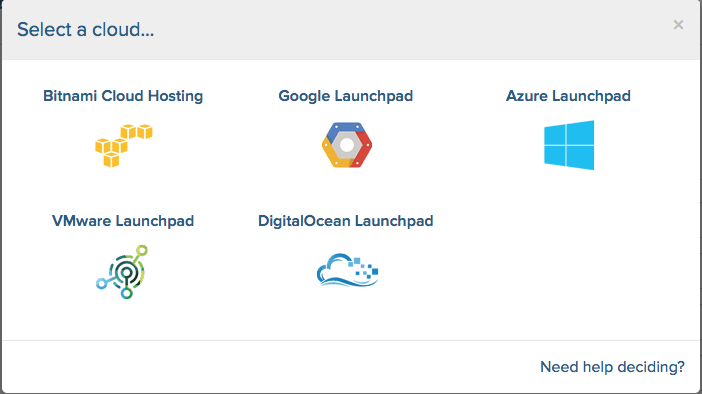
\includegraphics[width=\textwidth]{./03_Analyse/03_Bitnami/images/clouds}
  \caption{Cloud Anbieter}
\end{figure}

\newpage
\subsubsection{Bitnami Cloud Hosting\autocite{aws}}

Beim Bitnami Cloud Hosting steckt AWS dahinter, hier sind die meisten 
Einstellungen möglich im Vergleich zu den anderen Dashboards.

\subsubsection{Übersicht}
Kurze Übersicht über die möglichen Konfigurationen einer AWS Instanz.
\begin{figure}[!htbp]
  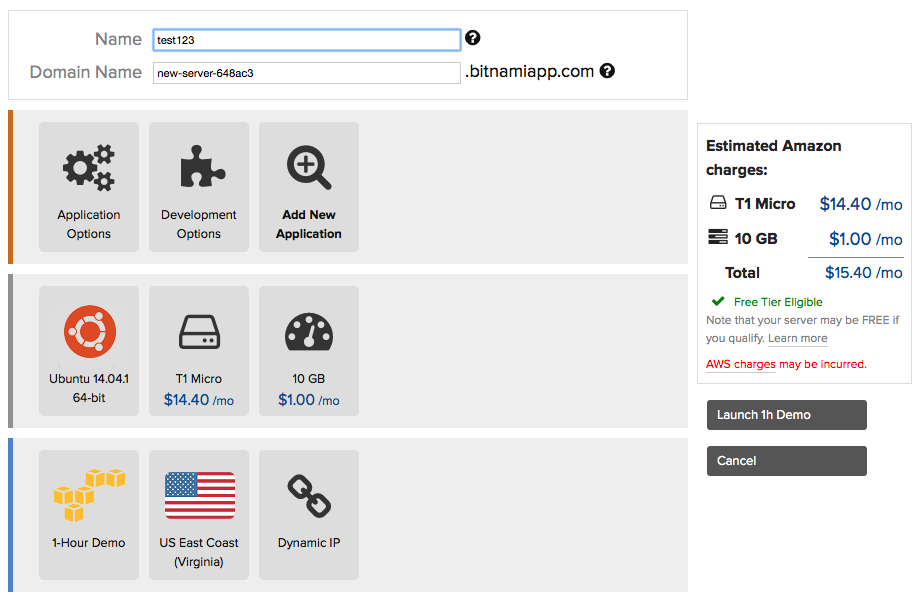
\includegraphics[width=\textwidth]{./03_Analyse/03_Bitnami/images/aws_overview}
  \caption{AWS Übersicht}
\end{figure}

\begin{figure}[!htbp]
  \centering
  \begin{subfigure}[b]{.49\textwidth}
\subsubsection{Applikationseinstellungen}
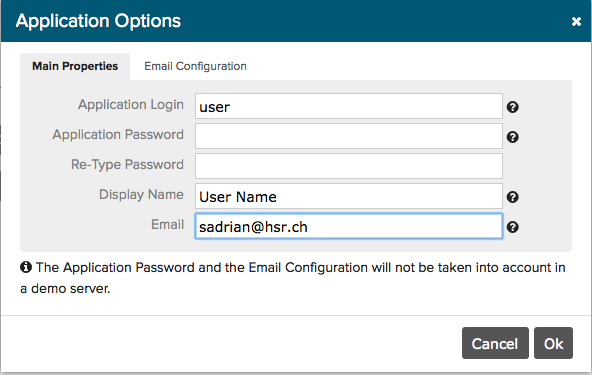
\includegraphics[width=\textwidth]{./03_Analyse/03_Bitnami/images/aws_application_options}
\caption{AWS Application Options}
\end{subfigure}
  \hfill
\begin{subfigure}[b]{.49\textwidth}
\subsubsection{Applikationsauswahl}
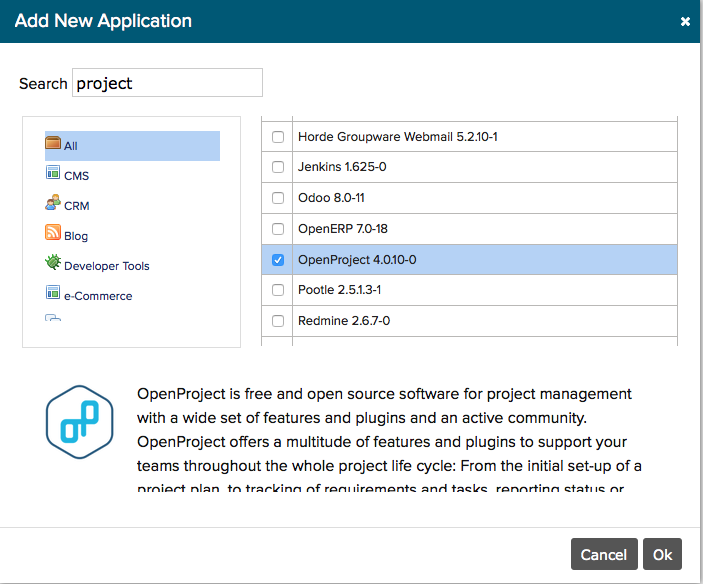
\includegraphics[width=\textwidth]{./03_Analyse/03_Bitnami/images/aws_add_application}
\caption{AWS Apllikationsauswahl}
\end{subfigure}
\caption{AWS Applikationseinstellungen}
\end{figure}

\begin{figure}[!htbp]
  \centering
\begin{subfigure}[b]{.49\textwidth}
\subsubsection{Betriebssystem}
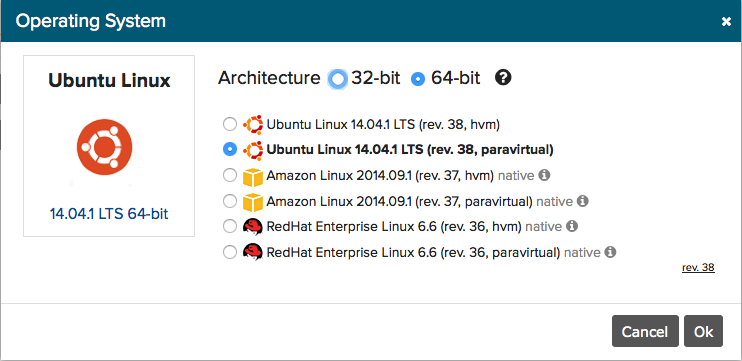
\includegraphics[width=\textwidth]{./03_Analyse/03_Bitnami/images/aws_operating_system}
\caption{AWS Betriebssystem}
\end{subfigure}
  \hfill
\begin{subfigure}[b]{.49\textwidth}
\subsubsection{Servertyp}
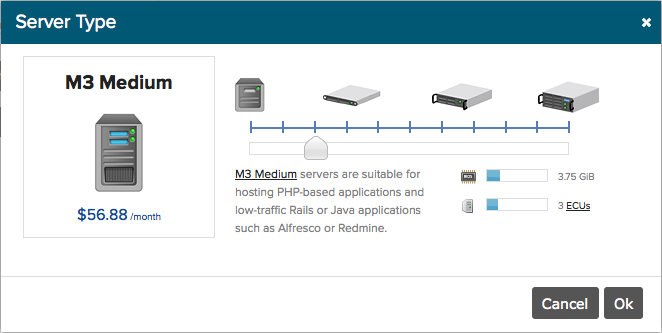
\includegraphics[width=\textwidth]{./03_Analyse/03_Bitnami/images/aws_servertype}
\caption{AWS Servertyp}
\end{subfigure}
\caption{AWS Betriebssystem und Servertyp}
\end{figure}

\begin{figure}[!htbp]
  \centering
  \begin{subfigure}[b]{.49\textwidth}
\subsubsection{Diskgrösse}
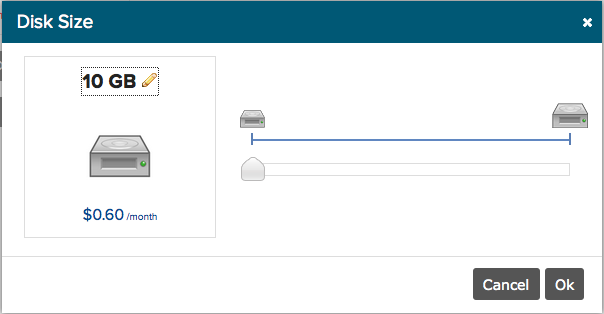
\includegraphics[width=\textwidth]{./03_Analyse/03_Bitnami/images/aws_disk}
\caption{AWS Diskgrösse}
\end{subfigure}
  \hfill
\begin{subfigure}[b]{.49\textwidth}
\subsubsection{Region,IP,Account}
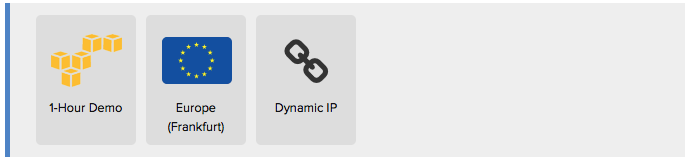
\includegraphics[width=\textwidth]{./03_Analyse/03_Bitnami/images/aws_random}
\caption{AWS Region,IP und Account}
\end{subfigure}
\caption{AWS Diskgrösse + Region,IP,Account}
\end{figure}

\newpage
 
\begin{figure}[!htbp]
   \centering
    \subsubsection{Management}
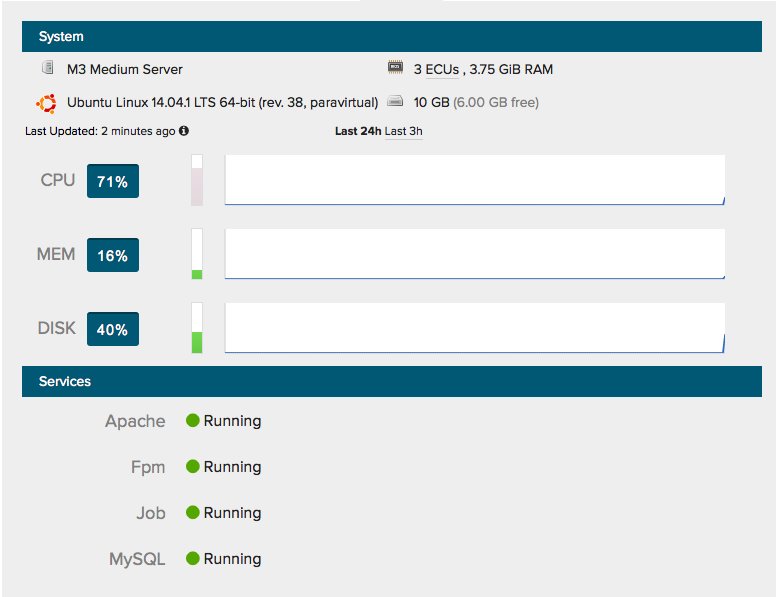
\includegraphics[width=.5\textwidth]{./03_Analyse/03_Bitnami/images/aws_resourcen}
\caption{AWS Management Ressourcen}
\end{figure}


\begin{figure}[!htbp]
 \centering
  \begin{subfigure}[b]{.49\textwidth}
\textbf{Ressourcen:}\\
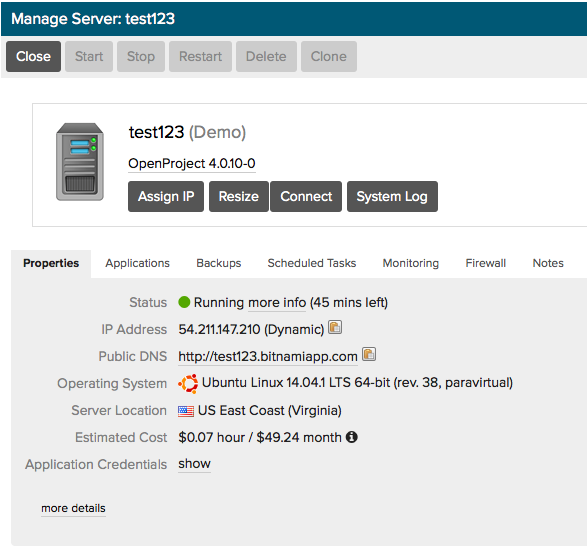
\includegraphics[width=\textwidth]{./03_Analyse/03_Bitnami/images/aws_managment}
\caption{AWS Server Management}
\end{subfigure}
  \hfill
 \begin{subfigure}[b]{.49\textwidth}
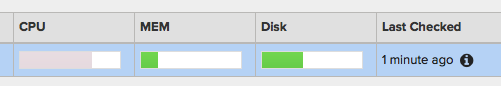
\includegraphics[width=\textwidth]{./03_Analyse/03_Bitnami/images/aws_resrouces}
\caption{AWS Server Ressourcen}
\end{subfigure}
\caption{AWS Ressourcen}
\end{figure}

\newpage
\subsubsection{Digitalocean Launchpad\autocite{digitalocean}}

\begin{figure}[!htbp]
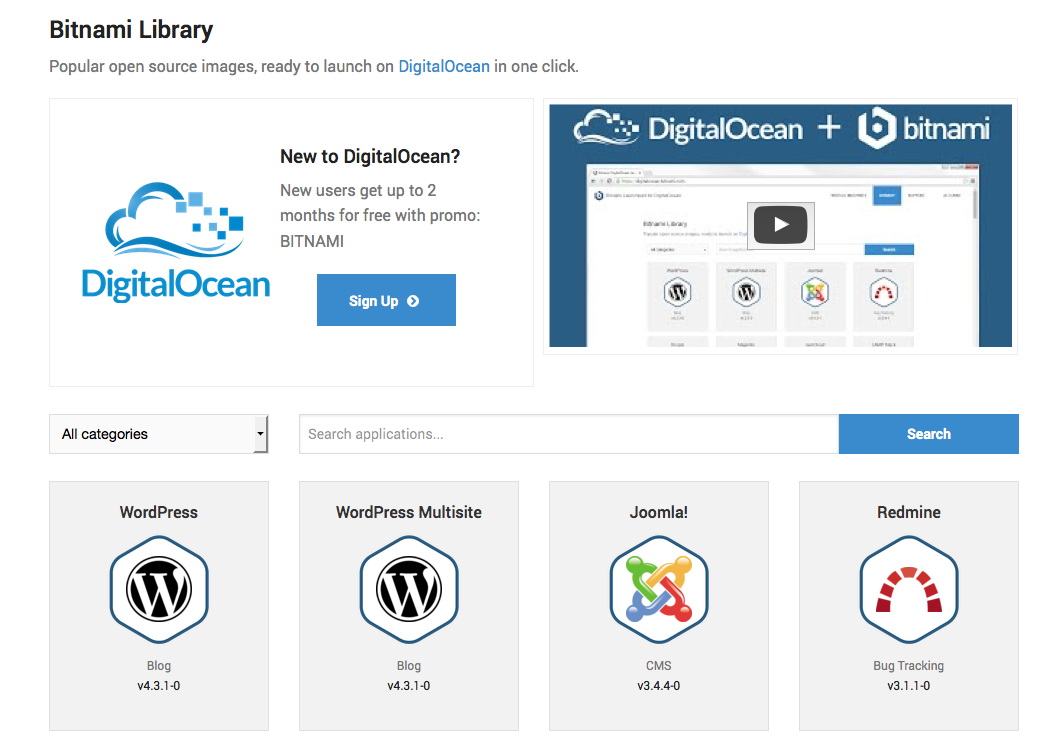
\includegraphics[width=\textwidth]{./03_Analyse/03_Bitnami/images/digitalocean_launchpad}
\caption{Digitalocean Launchpad}
\end{figure}

\newpage
\subsubsection{Authorize Application}
Um Instanzen erstellen zu können muss das Bitnami Dashboard Zugriff auf 
den User-Account beim Cloud Anbieter haben.

\begin{figure}[!htbp]
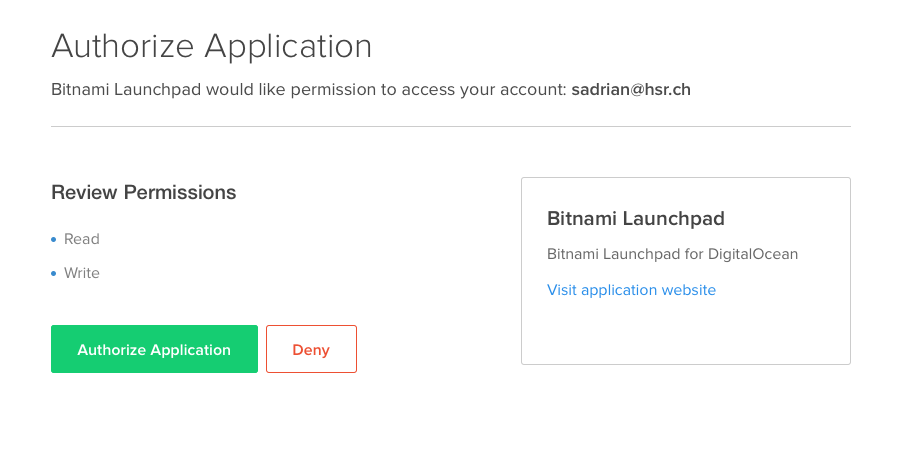
\includegraphics[width=0.8\textwidth]{./03_Analyse/03_Bitnami/images/digitalocean_authorize}
\caption{Digitalocean Applikation autorisieren}
\end{figure}




\begin{figure}[!htbp]
   \begin{subfigure}[b]{.49\textwidth}
\subsubsection{Instanzen}
Sobald eine Applikation ausgewählt wurde kann eine Instanz mit dem App gestartet 
werden, dabei kann noch die Instanzgrösse und der Standort gewählt werden.
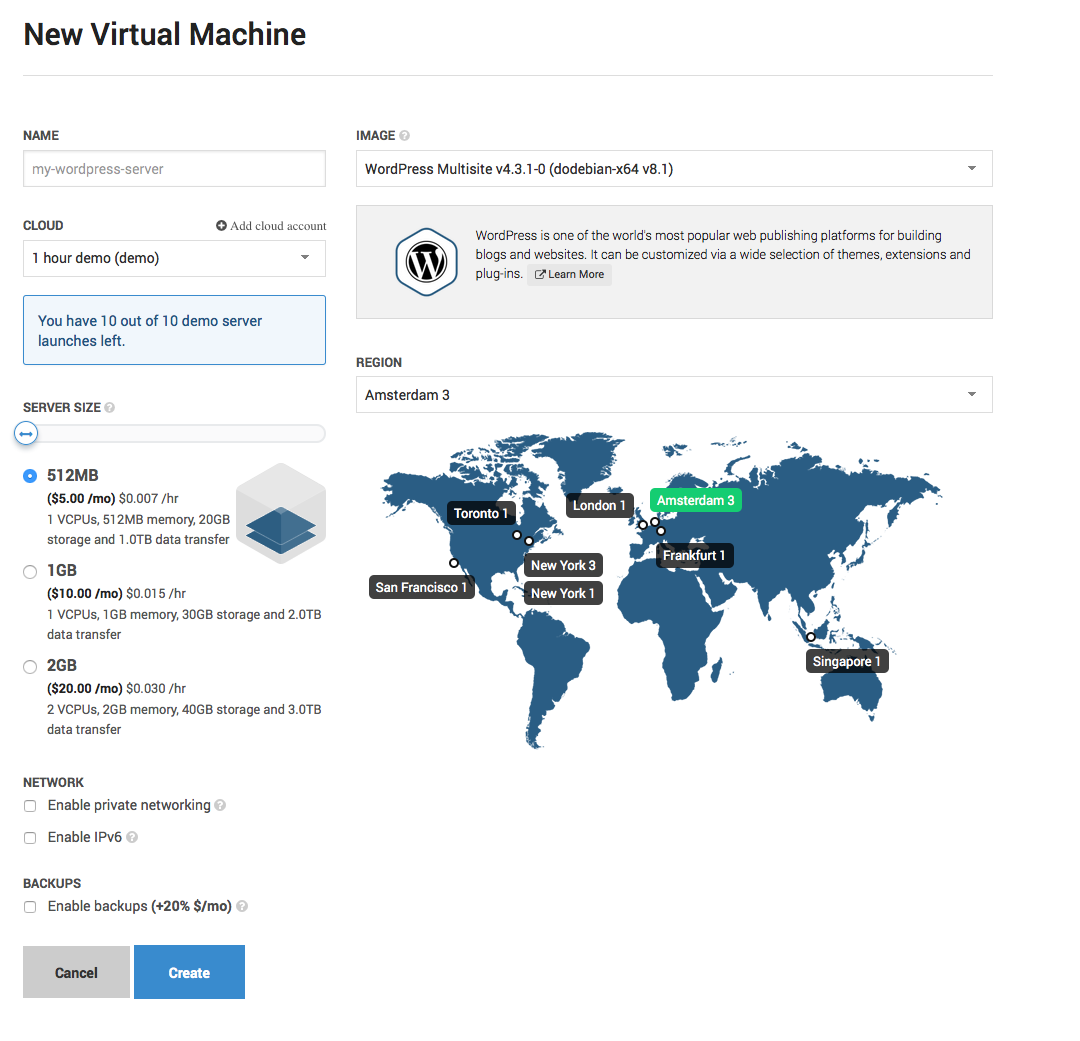
\includegraphics[width=\textwidth]{./03_Analyse/03_Bitnami/images/digitalocean_size}
\caption{Digitalocean Instanz}
\end{subfigure}
  \hfill
 \begin{subfigure}[b]{.49\textwidth}
  \subsubsection{Instanzinfos}
  Sobald die Instanz erstellt wurde lässt sich deren Status überprüfen + App spezifische 
Links werden gesetzt und Private Key/Public Key lassen sich herunterladen.\\
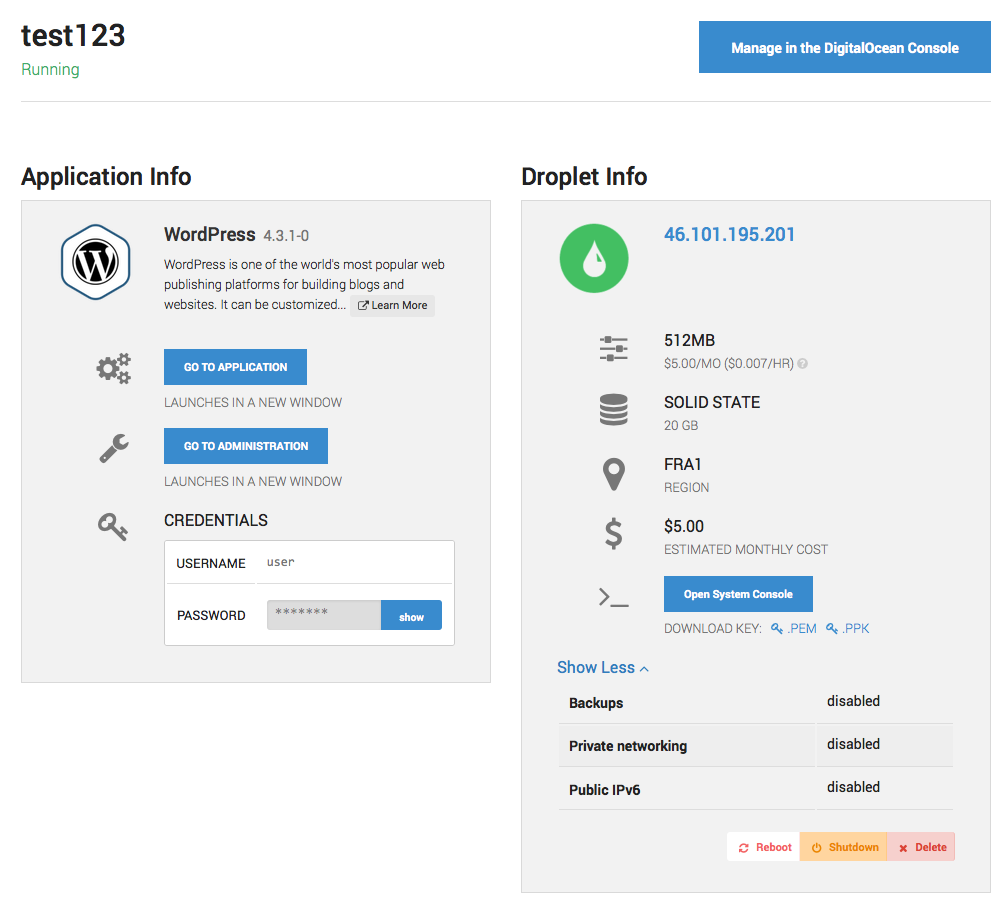
\includegraphics[width=\textwidth]{./03_Analyse/03_Bitnami/images/digitalocean_instanceinfo}
\caption{Digitalocean Instanzinfos}
\end{subfigure}
\caption{Digitalocean Instanz}
\end{figure}

\subsubsection{Cloud Accounts}
Es besteht die Möglichkeit mehrere Cloud Accounts in Bitnami zu hinterlegen.
\begin{figure}[!htbp]
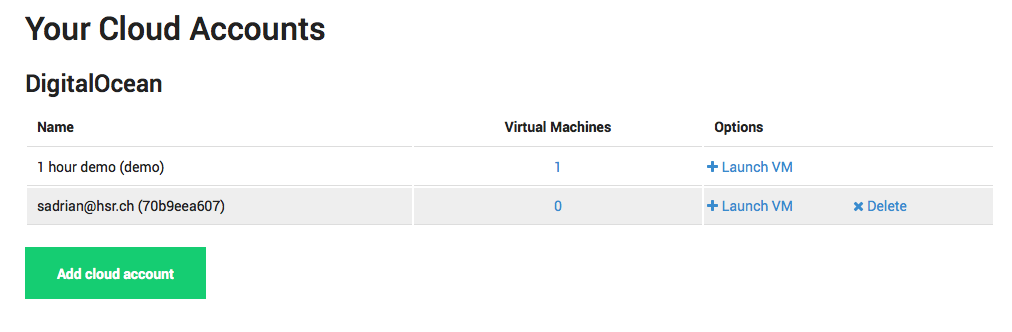
\includegraphics[width=\textwidth]{./03_Analyse/03_Bitnami/images/digitalocean_accounts}
\caption{Digitalocean Cloud Accounts}
\end{figure}



\begin{figure}[!htbp]
\centering
Und unter jedem Account können eigene VMs erstellt werden:\\
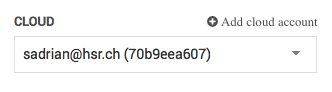
\includegraphics[width=0.5\textwidth]{./03_Analyse/03_Bitnami/images/digitalocean_account_specific}
\caption{Digitalocean Account spezifischische VMs}
\end{figure}

\begin{figure}[!htbp]
 \centering
Danach taucht die Instanz in der Übersicht auf:
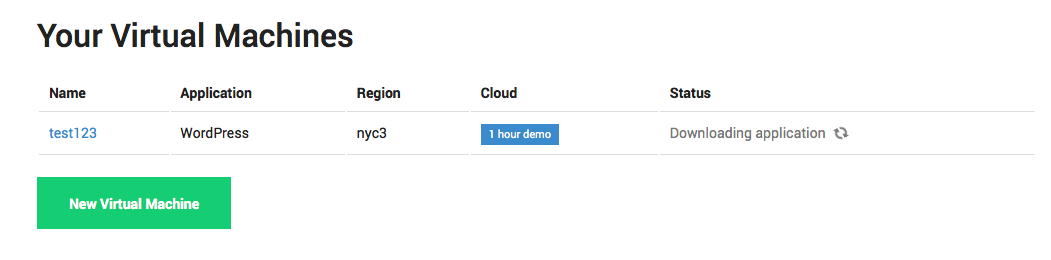
\includegraphics[width=\textwidth]{./03_Analyse/03_Bitnami/images/digitalocean_instances}
\caption{Digitalocean Instanzen}
\end{figure}

\newpage

\subsubsection{Azure Launchpad\autocite{azure}}
Beim Azure Launchpad wird wieder gleich vorgegangen, wie bei Digitalocean.
Nur das sich die Namen ändern (Bspw.: Bei Digitalocean Droplet, jetzt Server).
\newline
Ebenfalls ändern sich die Instanzgrössen, welche bei Azure anders als bei 
Digitalocean sind + wird bei Azure mit Subscriptions und nicht anhand von 
Accounts unterschieden.


\begin{figure}[!htbp]
\centering
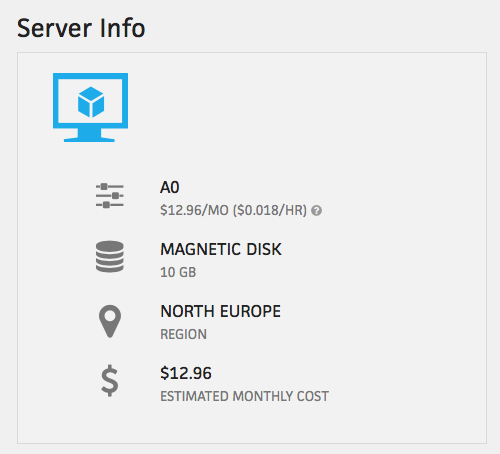
\includegraphics[width=0.4\textwidth]{./03_Analyse/03_Bitnami/images/azure_serverinfo}
\caption{Azure Serverinfo}
\end{figure}

\begin{figure}[!htbp]
 \begin{subfigure}[b]{.49\textwidth}
\subsubsection{Authorization:}
Bei Azure wird das Dashboard über ein Management Zertifikat autorisiert:
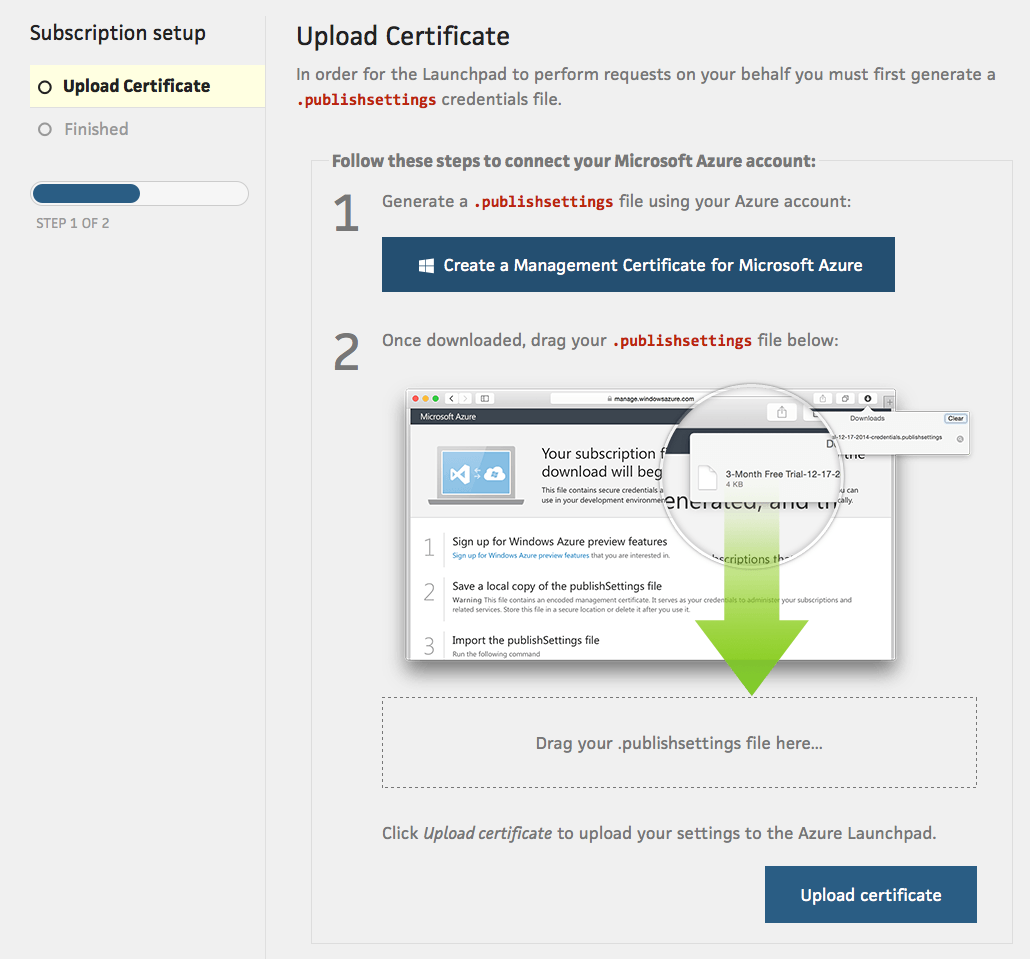
\includegraphics[width=\textwidth]{./03_Analyse/03_Bitnami/images/azure_authorize}
\caption{Azure Management Zertifikat}
\end{subfigure}
\hfill
 \begin{subfigure}[b]{.49\textwidth}
Danach werden die vorhandenen Subscriptions vom Azure Account eingebunden:
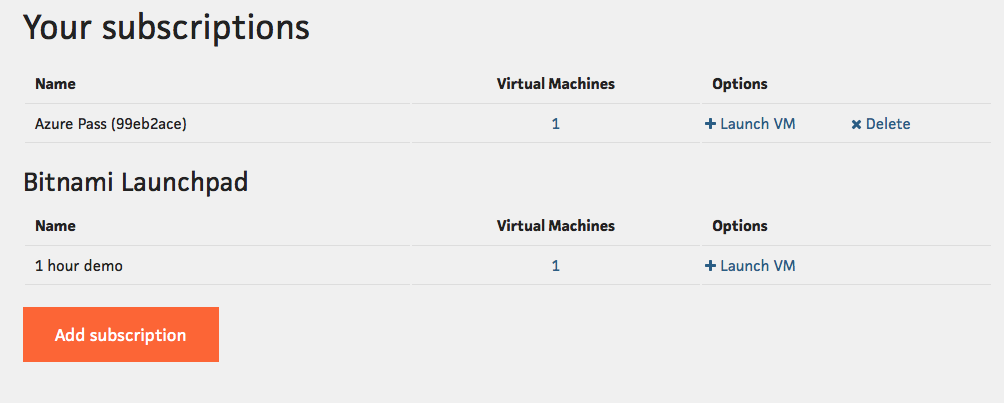
\includegraphics[width=\textwidth]{./03_Analyse/03_Bitnami/images/azure_subscriptions}
\caption{Azure Subscription}
\end{subfigure}
\caption{Azure Authorization}
\end{figure}


\begin{figure}[!htbp]
Sobald dann ein neuer Server erstellt wurde kann dieser auch wieder gelöscht 
werden und all dessen Infos eingesehen werden.\\
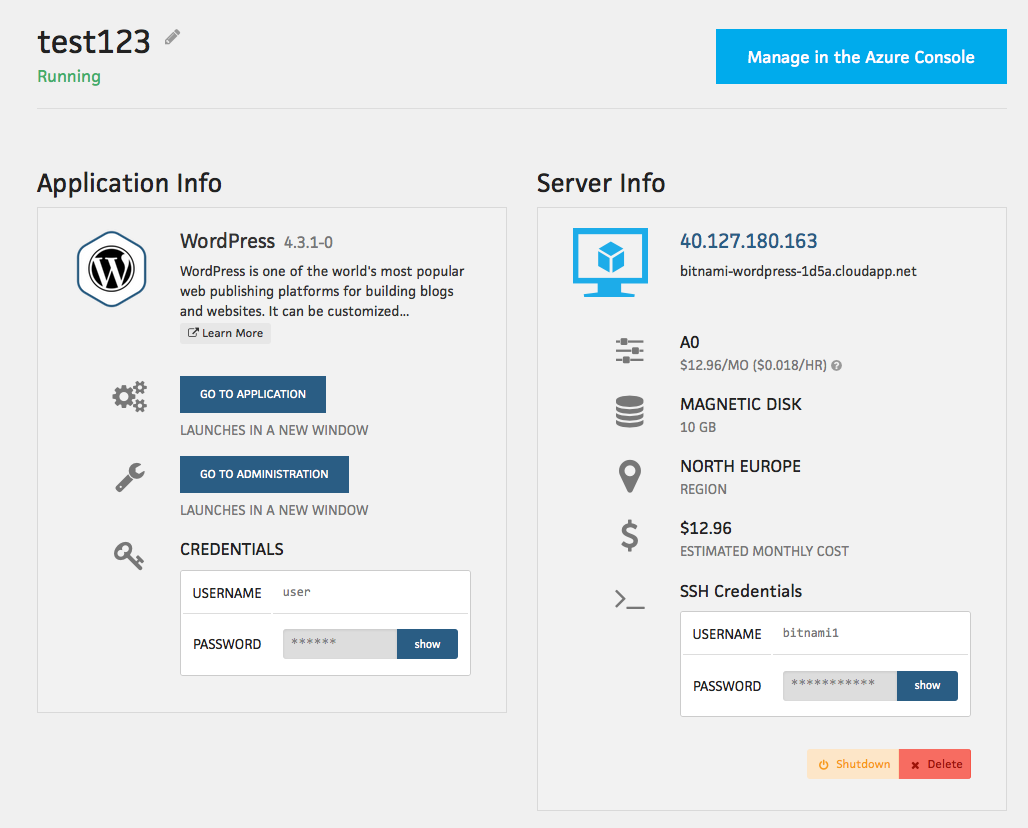
\includegraphics[width=\textwidth]{./03_Analyse/03_Bitnami/images/azure_instanceinfos}
\caption{Azure Instanzinfos}
\end{figure}

\newpage

\subsubsection{Google Launchpad\autocite{google}}

Beim Google Launchpad wieder dasselbe, wie bei Azure oder Digitalocean.
Hier wird einfach mit Projekten unterschieden (schliesslich können jedem Projekt mehrere Compute Instanzen 
oder andere Services angefügt werden).

\begin{figure}[!htbp]
  \centering
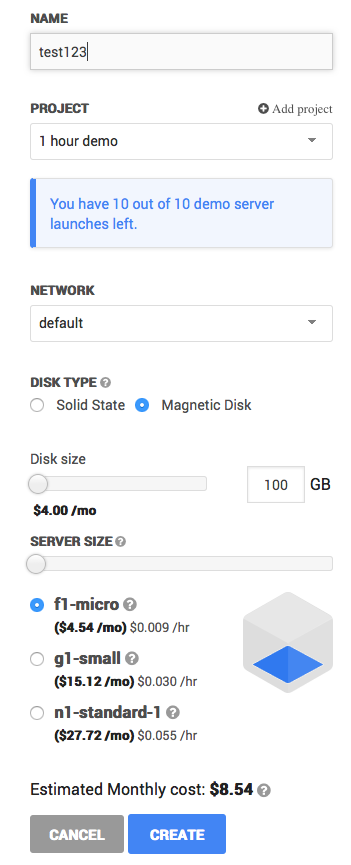
\includegraphics[width=0.4\textwidth]{./03_Analyse/03_Bitnami/images/google_instancereation}
\caption{Google Instanzerstellung}
\end{figure}

\newpage
\subsubsection{VMware Launchpad\autocite{vmware}}
Das VMware Launchpad kann für die VMware vCloud Air gebraucht werden und wieder 
die gleiche vorgehensweise, wie bei den anderen Anbietern.
\begin{figure}[!htbp]
   \begin{subfigure}[b]{.6\textwidth}

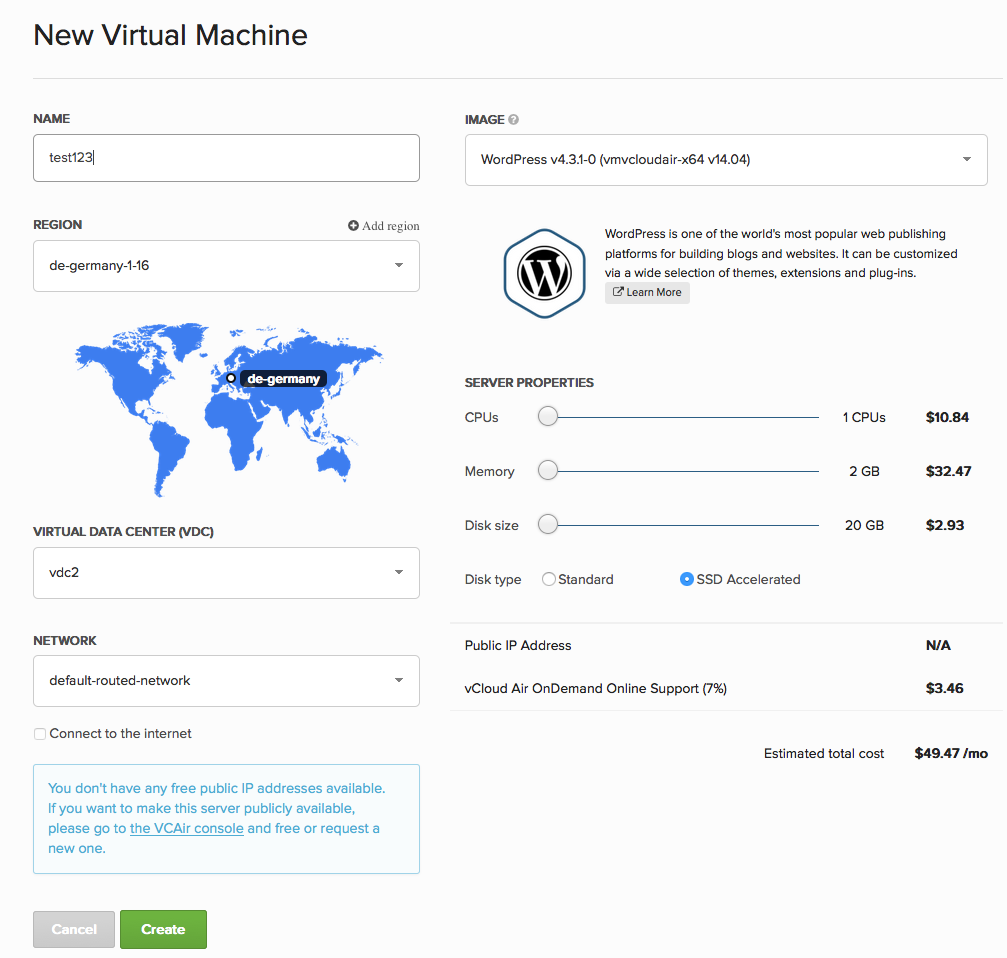
\includegraphics[width=\textwidth]{./03_Analyse/03_Bitnami/images/vmware_creation}
\caption{VMware Instanzerstellung}
   \end{subfigure}
     \hfill
   \begin{subfigure}[b]{.39\textwidth}
  \centering
\textbf{Infos:}\\
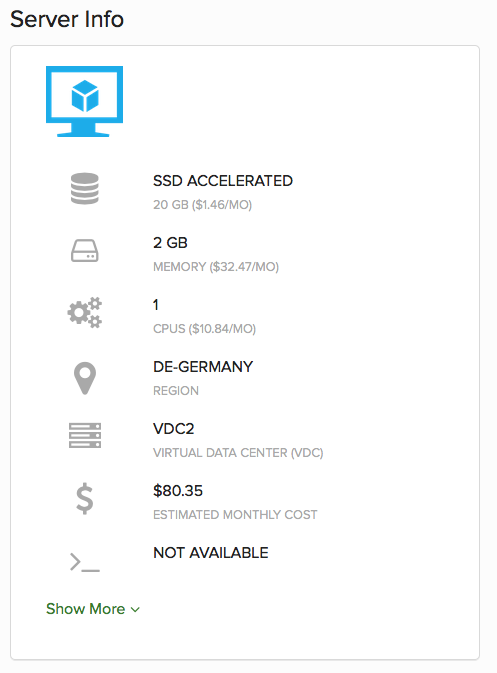
\includegraphics[width=\textwidth]{./03_Analyse/03_Bitnami/images/vmware_infos}
\caption{VMware Infos}
\end{subfigure}
   \caption{VMware Launchpad}
\end{figure}


  \subsection{Security}
  Da durch das zentrale zusammenfassen von mehreren Accounts auch immer 
Sicherheitsrisiken zu beachten sind, wird bei Bitnami zusätzlich zum normalen 
Benutzerpasswort auch noch ein Vaultpasswort gesetzt, welches wohl die 
Logindaten symmetrisch verschlüsselt und in einem ``Vault'' ablegt.

\begin{figure}[!htbp]
  \centering
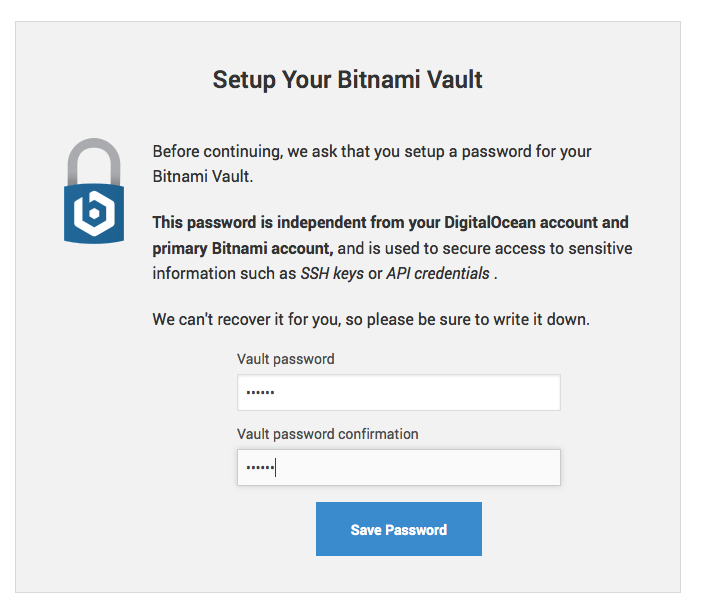
\includegraphics[width=0.6\textwidth]{./03_Analyse/03_Bitnami/images/bitnami_security}
\caption{Bitnami Security}
\end{figure}
\newpage

\subsection{Applikationen}
Die Applikationen können sich von Anbieter zu Anbieter unterscheiden, jedoch 
gibt es für sehr bekannte Applikationen (Bspw.: Wordpress) bei jedem ein 
Image.
Es besteht bereits eine sehr grosse Auswahl für sehr viel verschiedene Apps und 
es werden immer mehr, wodurch es immer einfacher wird schnell eine Applikation 
in der Public Cloud aufzusetzen.

\begin{figure}[!htbp]
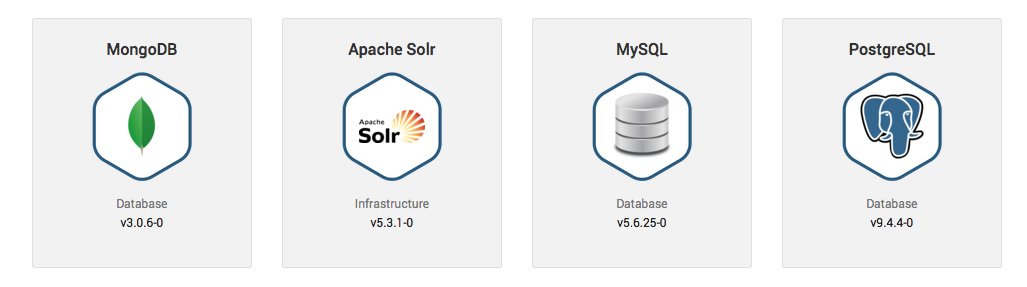
\includegraphics[width=\textwidth]{./03_Analyse/03_Bitnami/images/apps}
\caption{Applikationen}
\end{figure}

\newpage 
\section{Fazit}
Bitnami bietet einiges was Computing angeht und ist der einzig grössere 
Dashboard Anbieter, der mehrere verschiedene Public Cloud Anbieter unterstützt.
Allerdings fehlen verschiedene PaaS Angebote (Bspw.: Cloud SQL bei Google etc.), 
Bitnami ist daher nur für eigene VM Instanzen zu gebrauchen und nicht mit einer 
generellen Service Unterstützung konzipiert worden.
Das Dashboard bei Bitnami bietet jedenfalls einiges und gibt einem einen guten 
Überblick über seine eigenen abonnierten Services (VM Instanzen).
